% Die Links werden in config.tex angepasst
% Hier muss idR nichts geändert werden.

\ifkogwiss
    % FSK
    Die erste beruhigende Information: Du bist nicht allein! Es fangen noch viele andere Studierende dieses Semester im \abschluss{} \studiengang an.
    Für das Kennenlernen bieten wir als Fachschaft euch eine Reihe von verschiedensten Veranstaltungen an, die ihr mit Terminen auf den Folgeseiten findet.
    Darüber hinaus möchten wir euch mit einer Semestergruppe die Möglichkeit bieten, auch per Chat in direkten Kontakt miteinander zu treten.
    Dafür nutzen wir WhatsApp. Auch einige von uns FachschaftlerInnen sind dort erreichbar. Ihr könnt der Gruppe über den nachstehenden QR-Code beitreten:

    \begin{center}
        \ifmaster
            % Master
            {
                \color{green}
                \qrcode[height=38mm]{\GruppeKogniMaster} \\
            }
            \vspace*{0.3cm}
            {
                \footnotesize
                Kogni Master \ifsommersemester SoSe \else WiSe \fi \YEAR \\
                \url{\GruppeKogniMaster}
            }
        \else
            % Bachelor
            {
                \color{green}
                \qrcode[height=38mm]{\GruppeKogniBachelor} \\
            }
            \vspace*{0.3cm}
            {
                \footnotesize
                Kogni Bachelor \ifsommersemester SoSe \else WiSe \fi \YEAR \\
                \url{\GruppeKogniBachelor}
            }
        \fi
    \end{center}

    % Kognis nutzen WhatsApp :')
    %Falls ihr euch fragt: \glqq Warum nicht WhatsApp?\grqq. Ganz einfach: Wir als Informatik-Fachschaft sehen es als Teil unserer Aufgabe, für digitale Souveränität einzutreten. 
    %Daher möchten wir in keinster Weise politisch und sicherheitstechnisch fragwürdige Plattformen wie WhatsApp bzw. Meta unterstützen.
    %Signal dagegen ist gemeinnützig, werbefrei und finanziert sich überwiegend durch Spenden statt durch die Auswertung von Nutzerdaten. Außerdem ist es Open Source Software.

    An dieser Stelle möchten wir außerdem einen kurzen Warnhinweis zur Plattform \textit{ersti-gruppen.de} aussprechen.
    Es tauchen immer wieder Hinweise dazu auf, dass die Betreiber dieser Plattform die dort gelisteten Gruppen auch zur Verbreitung von eigenen, kommerziellen Inhalten nutzen; teilweise werden auch WhatsApp-Business-Accounts und Chatbots verwendet.
    Wir möchten daher mit der oben verlinkten Gruppe eine sichere und werbefreie Alternative bieten. Mit \textit{ersti-gruppen.de} stehen wir in keinster Weise in Verbindung.

    \begin{center}
        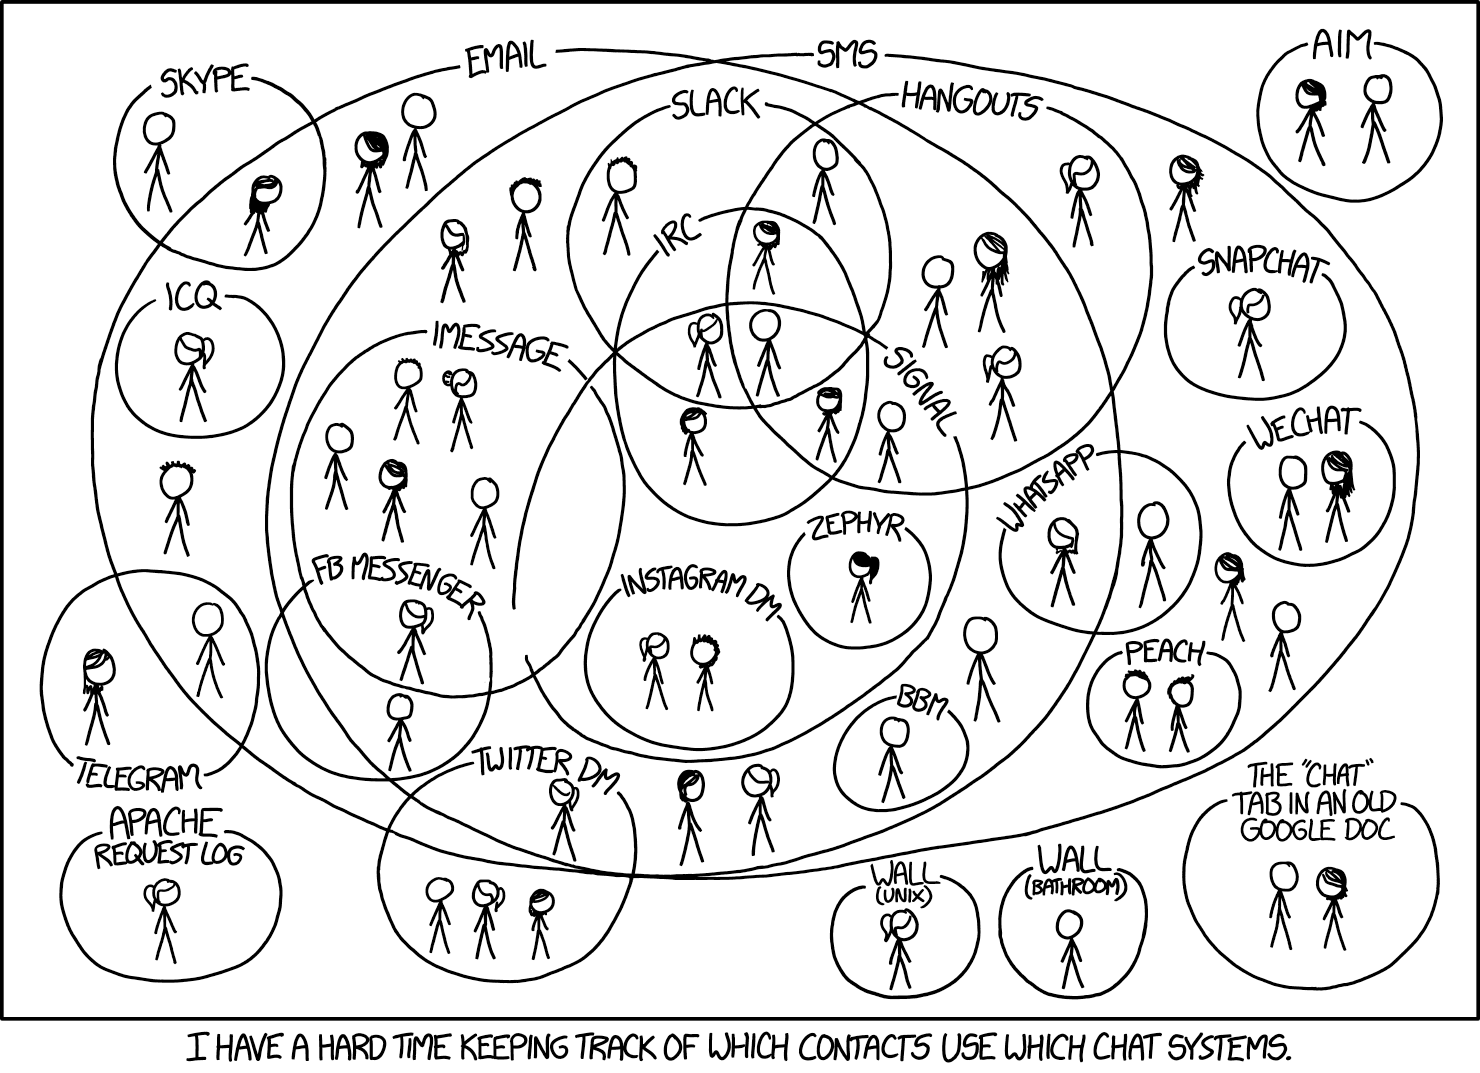
\includegraphics[height=60mm, keepaspectratio=true]{media/xkcd_chats.png} \\
        {
            \tiny
            Quelle: \href{https://xkcd.com/1810}{xkcd.com}, Comic \#1810
        }
    \end{center}
\else
    % FSI
    \ifml
        % Englisch (MSc Machine Learning)
        The first reassuring piece of information: You are not alone! Many other students are also starting the \abschluss{} \studiengang this semester.
        To help you get to know each other, we as the student council have organized a wide range of events. You can find the dates on the following pages.
        In addition, we would like to offer you the opportunity to get in direct contact with each other via chat in a semester group.
        For this, we use the Signal messenger. Some of us from the student council are also available there. You can join the group using the QR code below:

        \begin{center}
            % ML immer Master
            {
                \color{navy}
                \qrcode[height=38mm]{\GruppeInfoMaster} \\
            }
            \vspace*{0.3cm}
            {
                \footnotesize
                Computer Science Master \ifsommersemester Summer Term \else Winter Term \fi \YEAR \\
                \url{\GruppeInfoMaster}
            }
        \end{center}

        If you are wondering: \glqq Why not WhatsApp?\grqq. Quite simply: As the Computer Science student council, we consider it part of our responsibility to advocate for digital sovereignty.
        Therefore, we do not want to support platforms such as WhatsApp or Meta, which we consider questionable from both a political and security perspective.
        Signal, on the other hand, is a non-profit, ad-free service and is funded primarily through donations rather than through the exploitation of user data. It is also open-source software.
        
        At this point, we would also like to give a brief warning regarding the platform \textit{ersti-gruppen.de}.
        There have repeatedly been reports that the operators of this platform also use the groups listed there to distribute their own commercial content; in some cases, WhatsApp Business accounts and chatbots are also used.
        With the Signal group linked above, we therefore want to provide a secure and ad-free alternative. We are in no way affiliated with \textit{ersti-gruppen.de}.

        \begin{center}
            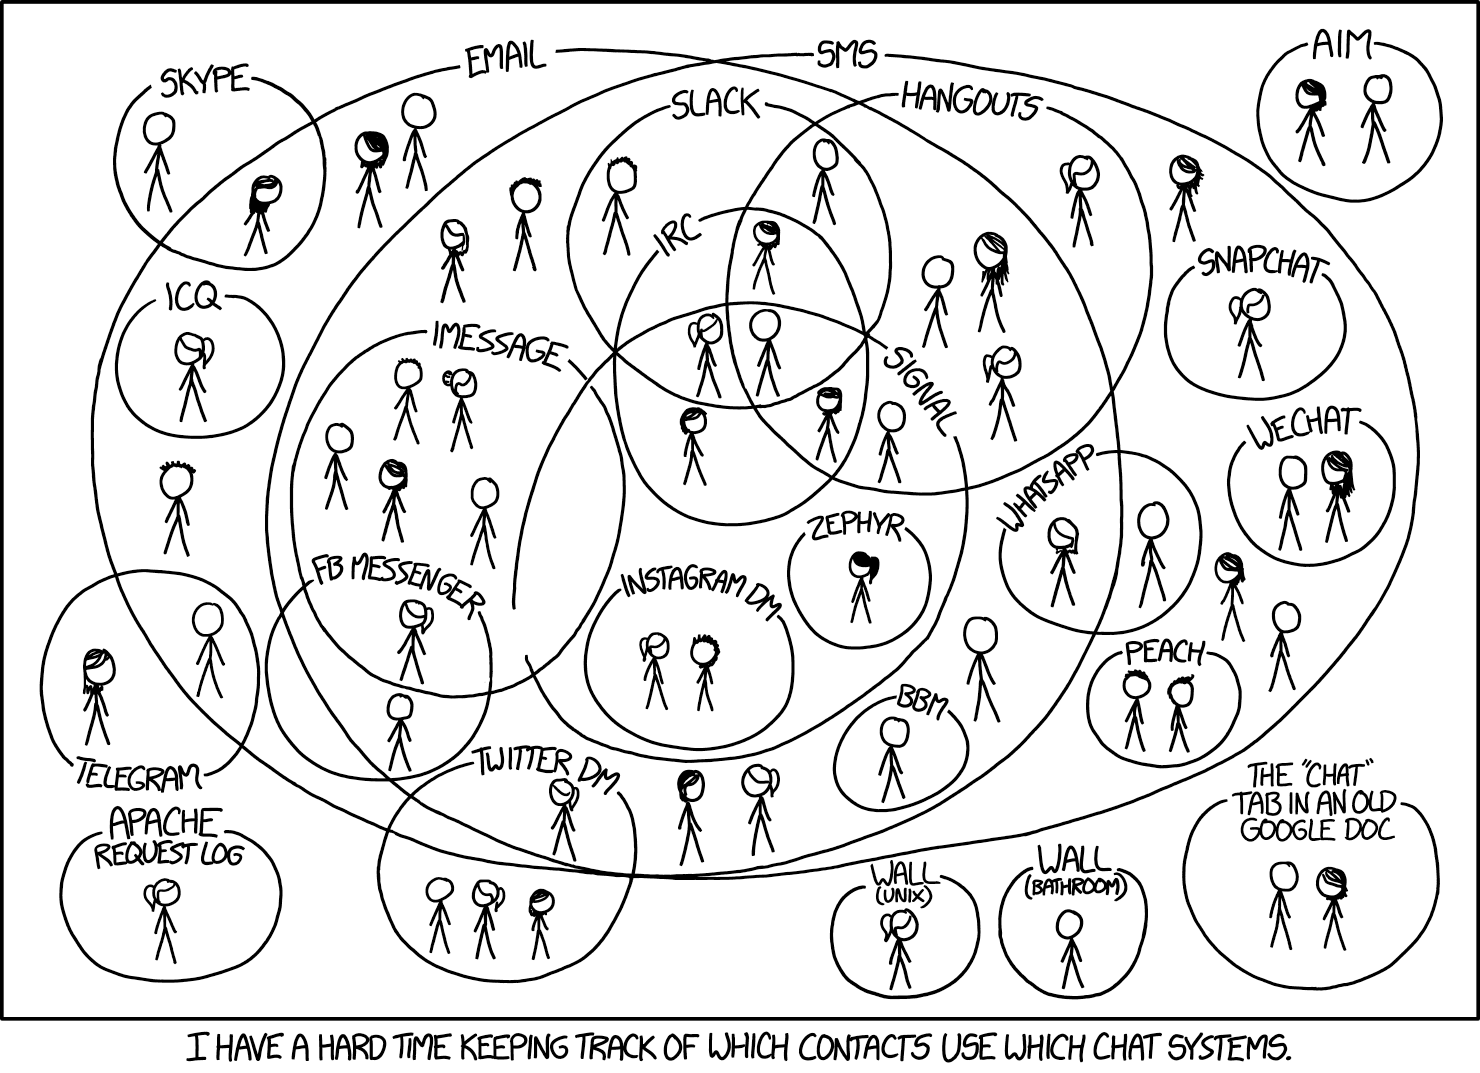
\includegraphics[height=60mm, keepaspectratio=true]{media/xkcd_chats.png} \\
            {
                \tiny
                Source: \href{https://xkcd.com/1810}{xkcd.com}, Comic \#1810
            }
        \end{center}
    \else
        % Deutsch (alles andere lol)
        Die erste beruhigende Information: Du bist nicht allein! Es fangen noch viele andere Studierende dieses Semester im \abschluss{} \studiengang an.
        Für das Kennenlernen bieten wir als Fachschaft euch eine Reihe von verschiedensten Veranstaltungen an, die ihr mit Terminen auf den Folgeseiten findet.
        Darüber hinaus möchten wir euch mit einer Semestergruppe die Möglichkeit bieten, auch per Chat in direkten Kontakt miteinander zu treten.
        Dafür nutzen wir den Messenger Signal. Auch einige von uns FachschaftlerInnen sind dort erreichbar. Ihr könnt der Gruppe über den nachstehenden QR-Code beitreten:

        \begin{center}
            \ifmaster
                % Master
                {
                    \color{navy}
                    \qrcode[height=38mm]{\GruppeInfoMaster} \\
                }
                \vspace*{0.3cm}
                {
                    \footnotesize
                    *-Informatik Master \ifsommersemester SoSe \else WiSe \fi \YEAR \\
                    \url{\GruppeInfoMaster}
                }
            \else
                % Bachelor
                {
                    \color{navy}
                    \qrcode[height=38mm]{\GruppeInfoBachelor} \\
                }
                \vspace*{0.3cm}
                {
                    \footnotesize
                    *-Informatik Bachelor \ifsommersemester SoSe \else WiSe \fi \YEAR \\
                    \url{\GruppeInfoBachelor}
                }
            \fi
        \end{center}

        Falls ihr euch fragt: \glqq Warum nicht WhatsApp?\grqq. Ganz einfach: Wir als Informatik-Fachschaft sehen es als Teil unserer Aufgabe, für digitale Souveränität einzutreten. 
        Daher möchten wir in keinster Weise politisch und sicherheitstechnisch fragwürdige Plattformen wie WhatsApp bzw. Meta unterstützen.
        Signal dagegen ist gemeinnützig, werbefrei und finanziert sich überwiegend durch Spenden statt durch die Auswertung von Nutzerdaten. Außerdem ist es Open Source Software.

        An dieser Stelle möchten wir außerdem einen kurzen Warnhinweis zur Plattform \textit{ersti-gruppen.de} aussprechen.
        Es tauchen immer wieder Hinweise dazu auf, dass die Betreiber dieser Plattform die dort gelisteten Gruppen auch zur Verbreitung von eigenen, kommerziellen Inhalten nutzen; teilweise werden auch WhatsApp-Business-Accounts und Chatbots verwendet.
        Wir möchten daher mit der oben verlinkten Signal-Gruppe eine sichere und werbefreie Alternative bieten. Mit \textit{ersti-gruppen.de} stehen wir in keinster Weise in Verbindung.

        \begin{center}
            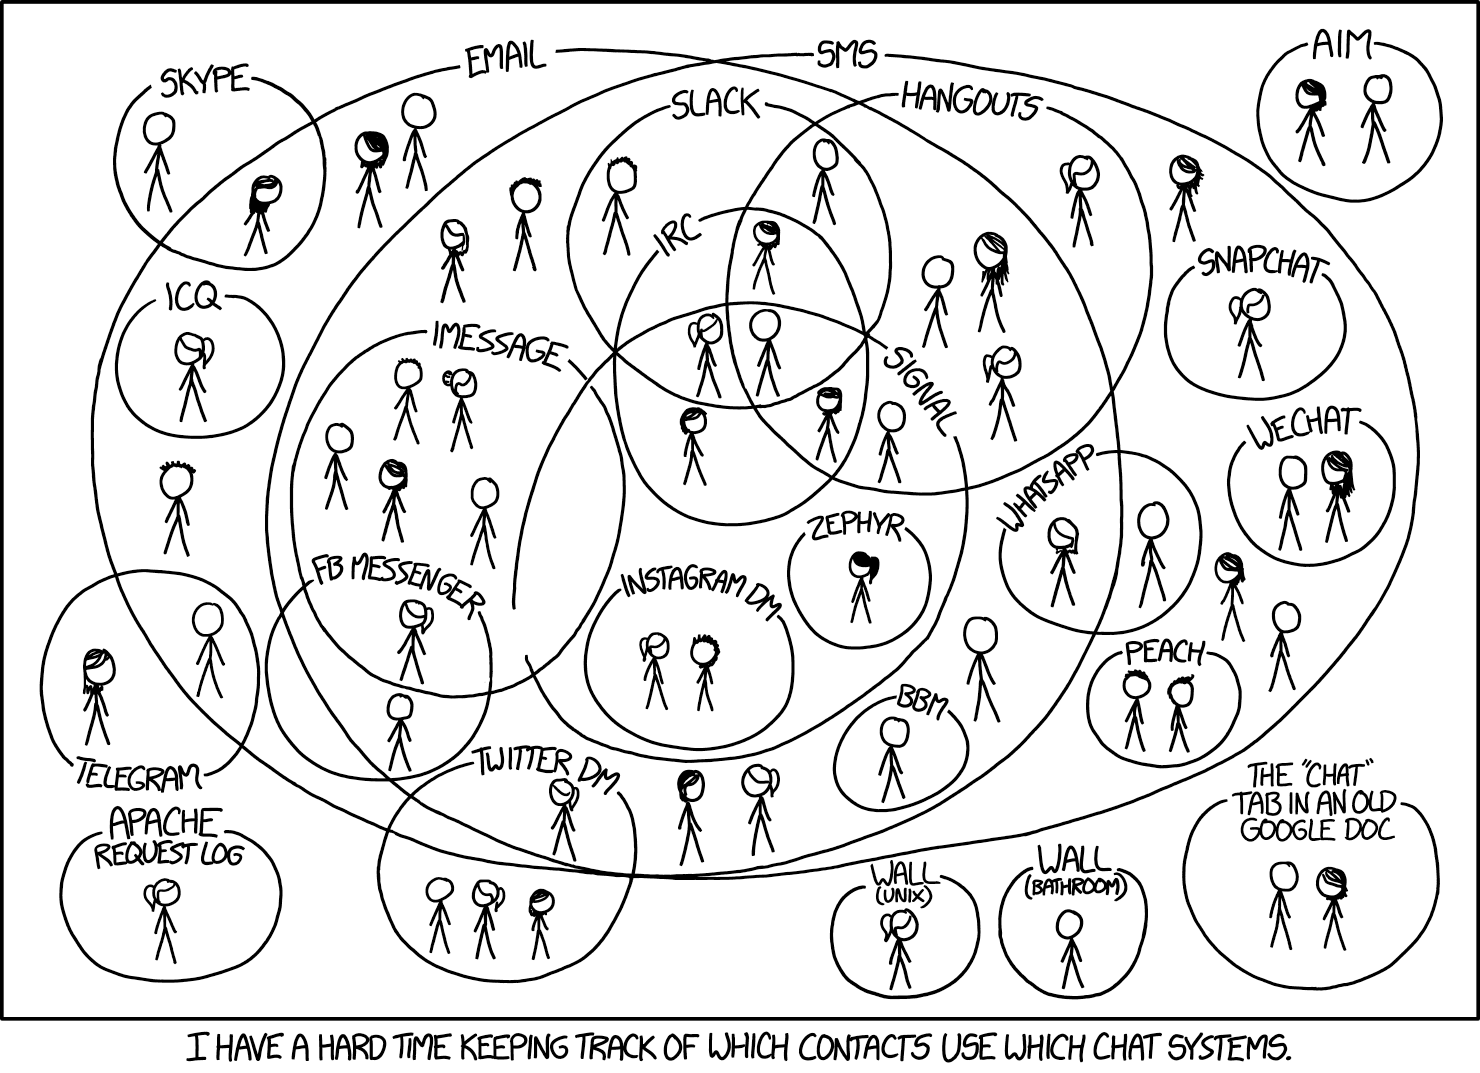
\includegraphics[height=60mm, keepaspectratio=true]{media/xkcd_chats.png} \\
            {
                \tiny
                Quelle: \href{https://xkcd.com/1810}{xkcd.com}, Comic \#1810
            }
        \end{center}
    \fi
\fi